\documentclass[12pt]{article}
\usepackage[utf8]{inputenc}
\newenvironment{sol}[1][Solution]{\begin{trivlist}\item[\hskip\labelsep {\bfseries #1:}]}{\end{trivlist}}
\usepackage[margin=1in]{geometry} 
\usepackage{amsmath,amsthm,amssymb}
\usepackage{color}
\usepackage{minted}
\usepackage{graphicx}
\title{Southern Methodist University \\
Bobby B. Lyle School of Engineering Department of Computer Science \\
Homework 6
}
\usepackage{times,url}   
\author{Operating System and Software System \\
Name: Bingying Liang 
\\ ID: 48999397\\ 
Email: bingyingl@smu.edu \\ 
CS7343 Distance}
\date{Apr 29 2023}

\begin{document}
\maketitle
\begin{itemize}
    \item\textbf{All students who are signed for this course at the CS 7343 must answer both questions.}
    \item \textbf{All students who are signed for this course at the CS 5343 must answer exactly one question.}
\end{itemize}

\begin{enumerate}
    \item Consider the following snapshot of a system (P=Process, R=Resource) :
    \begin{center}
        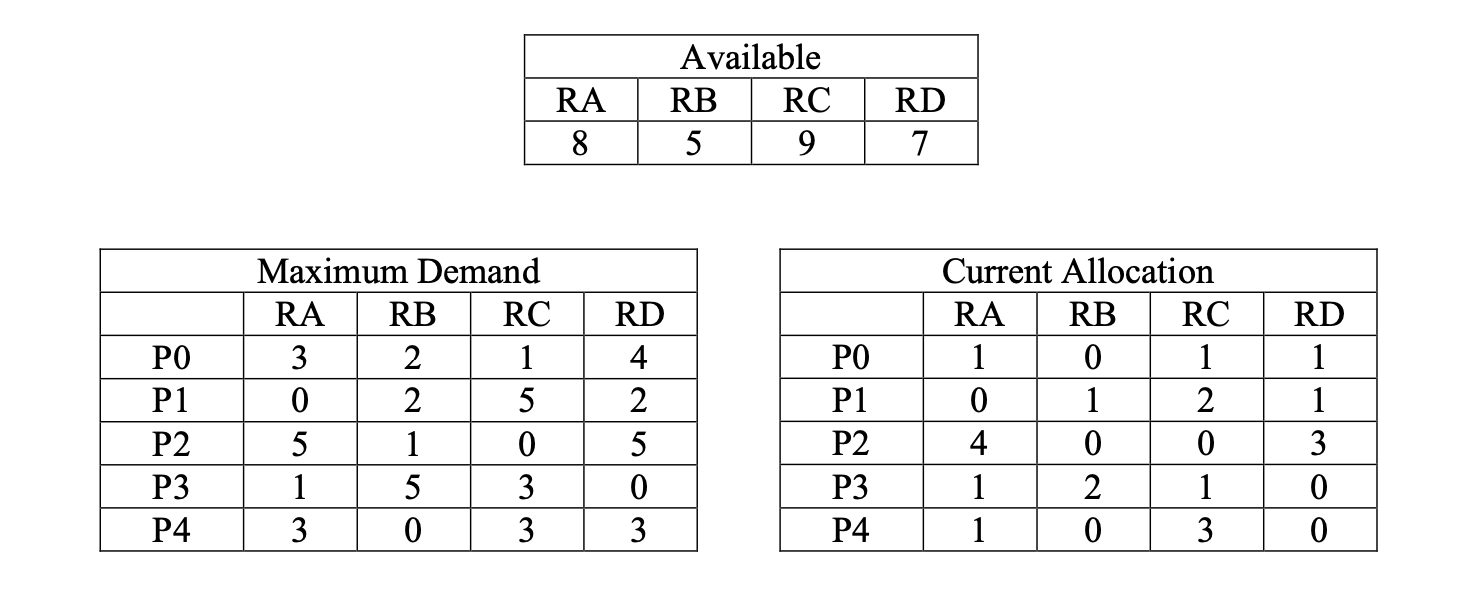
\includegraphics[width=0.9\textwidth]{p1.png}
    \end{center}
    Answer the following questions using banker’s algorithm:
    \begin{enumerate}
        \item Calculate the Needs matrix:
        \begin{sol}
        \hspace*{\fill}
            \begin{center}
                \begin{tabular}{|c|c|c|c|c|}
                \hline
                \multicolumn{5}{|c|}{Needs}\\
                \hline
                     & RA & RB & RC & RD \\
                     \hline
                    P0 & 2 & 2 &0 &3 \\
                    \hline
                    P1&0 &1 &3 &1 \\
                    \hline
                    P2&1 &1 &0 &2 \\
                    \hline
                    P3 & 0&3 &2 &0\\
                    \hline
                    P4 & 2&0 &0 &3 \\
                    \hline
                \end{tabular}
            \end{center}
        \end{sol}
        \item Is the system in a safe state? If so, show a safe order in which the processes can run.
        \begin{sol}
            \hspace*{\fill}\\
            Yes. Because the available after allocation is in the following as the question mentioned which are satisfy the processes. \\
            \begin{center}
                \begin{tabular}{|c|c|c|c|}
                \hline
                \multicolumn{4}{|c|}{Available}\\
                \hline
                   RA & RB & RC & RD  \\
                \hline
                   8 & 5 & 9 & 7   \\
                \hline
                \end{tabular}
            \end{center}
            For this moment it satisfy the P0, P1, P2, P3, P4 needs. Then we can go P0 first.
            \begin{itemize}
                \item P0 allocation and finish, the available:
                   \begin{center}
                \begin{tabular}{|c|c|c|c|}
                \hline
                \multicolumn{4}{|c|}{Available}\\
                \hline
                   RA & RB & RC & RD  \\
                \hline
                   9 & 5 & 10 & 8   \\
                \hline
                \end{tabular}
                          \end{center}
                \item P1 allocation and finish, the available:
                                   \begin{center}
                \begin{tabular}{|c|c|c|c|}
                \hline
                \multicolumn{4}{|c|}{Available}\\
                \hline
                   RA & RB & RC & RD  \\
                \hline
                   9 & 6 & 12 & 9   \\
                \hline
                \end{tabular}
                \end{center}

                \item P2 allocation and finish, the available:
                \begin{center}
                    
                 \begin{tabular}{|c|c|c|c|}
                \hline
                \multicolumn{4}{|c|}{Available}\\
                \hline
                   RA & RB & RC & RD  \\
                \hline
                   13 & 6 & 12 & 12   \\
                \hline
                \end{tabular}
                \end{center}

                \item P3 allocation and finish, the available:
                \begin{center}
                    
                 \begin{tabular}{|c|c|c|c|}
                \hline
                \multicolumn{4}{|c|}{Available}\\
                \hline
                   RA & RB & RC & RD  \\
                \hline
                   14 & 8 & 13 & 12   \\
                \hline
                \end{tabular}
                \end{center}

                \item P4 allocation and finish, the available:
                \begin{center}
                    
                 \begin{tabular}{|c|c|c|c|}
                \hline
                \multicolumn{4}{|c|}{Available}\\
                \hline
                   RA & RB & RC & RD  \\
                \hline
                   15 & 8 & 16 & 12   \\
                \hline
                \end{tabular}
                \end{center}
                          
            \end{itemize}
            All processes finshes.

            Therefore, A safe order can be P0, P1, P2, P3, P4.
            
        \end{sol}
        \item Can a request of one instance of RA by Process P0 be granted safely according to Banker’s
algorithm? Why/Why not?
        \begin{sol}
          Yes. \\
          When one instance of RA by process P0 be granted safely will become in the following:
                      \begin{center}
                \begin{tabular}{|c|c|c|c|c|}
                \hline
                \multicolumn{5}{|c|}{Needs}\\
                \hline
                     & RA & RB & RC & RD \\
                     \hline
                    P0 & \textcolor{red}{1} & 2 &0 &3 \\
                    \hline
                    P1&0 &1 &3 &1 \\
                    \hline
                    P2&1 &1 &0 &2 \\
                    \hline
                    P3 & 0&3 &2 &0\\
                    \hline
                    P4 & 2&0 &0 &3 \\
                    \hline
                \end{tabular}
                                \begin{tabular}{|c|c|c|c|c|}
                \hline
                \multicolumn{5}{|c|}{Current Allocation}\\
                \hline
                     & RA & RB & RC & RD \\
                     \hline
                    P0 & \textcolor{red}{2} & 0 &1 &1 \\
                    \hline
                    P1&0 &1 &2 &1 \\
                    \hline
                    P2&4 &0 &0 &3 \\
                    \hline
                    P3 & 1&2 &1 &0\\
                    \hline
                    P4 & 1&0 &3&0 \\
                    \hline
                \end{tabular}
                                \begin{tabular}{|c|c|c|c|}
                \hline
                \multicolumn{4}{|c|}{Available}\\
                \hline
                   RA & RB & RC & RD  \\
                \hline
                   \textcolor{red}{7} & 5 & 9 & 7   \\
                \hline
                \end{tabular}
            \end{center} 
           For this moment it satisfy the P0, P1, P2, P3, P4 needs. Then we can go P0 first.
                       \begin{itemize}
                \item P0 allocation and finish, the available:
                   \begin{center}
                \begin{tabular}{|c|c|c|c|}
                \hline
                \multicolumn{4}{|c|}{Available}\\
                \hline
                   RA & RB & RC & RD  \\
                \hline
                   9 & 5 & 10 & 8   \\
                \hline
                \end{tabular}
                          \end{center}
                \item P1 allocation and finish, the available:
                                   \begin{center}
                \begin{tabular}{|c|c|c|c|}
                \hline
                \multicolumn{4}{|c|}{Available}\\
                \hline
                   RA & RB & RC & RD  \\
                \hline
                   9 & 6 & 12 & 9   \\
                \hline
                \end{tabular}
                \end{center}

                \item P2 allocation and finish, the available:
                \begin{center}
                    
                 \begin{tabular}{|c|c|c|c|}
                \hline
                \multicolumn{4}{|c|}{Available}\\
                \hline
                   RA & RB & RC & RD  \\
                \hline
                   13 & 6 & 12 & 12   \\
                \hline
                \end{tabular}
                \end{center}

                \item P3 allocation and finish, the available:
                \begin{center}
                    
                 \begin{tabular}{|c|c|c|c|}
                \hline
                \multicolumn{4}{|c|}{Available}\\
                \hline
                   RA & RB & RC & RD  \\
                \hline
                   14 & 8 & 13 & 12   \\
                \hline
                \end{tabular}
                \end{center}

                \item P4 allocation and finish, the available:
                \begin{center}
                    
                 \begin{tabular}{|c|c|c|c|}
                \hline
                \multicolumn{4}{|c|}{Available}\\
                \hline
                   RA & RB & RC & RD  \\
                \hline
                   15 & 8 & 16 & 12   \\
                \hline
                \end{tabular}
                \end{center}
                          
            \end{itemize}

           Therefore, a request of one instance of RA by Process P0 can be granted safely according to
Banker’s algorithm.
        \end{sol}

    \end{enumerate}

    \item At an instant, the resource allocation state in a system is as follows:
    4 processes P1–P4\\
    4 resource types: R1–R4\\
    R1 (5 instances), R2 (3 instances), R3 (3 instances), R4 (3 instance)\\
    Snapshot at time T0:\\
        \begin{center}
        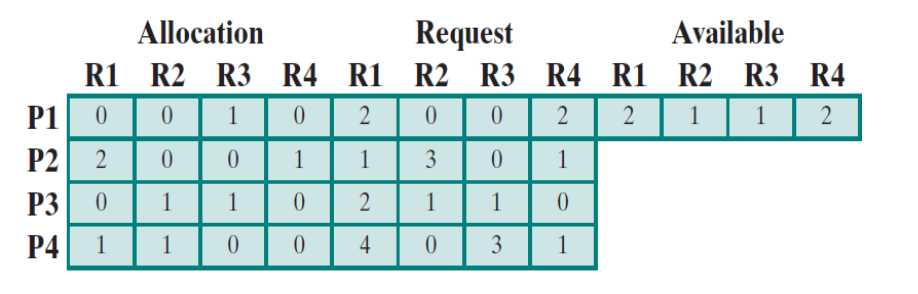
\includegraphics[width=0.7\textwidth]{p2.png}
    \end{center}
    Run the deadlock detection algorithm and test whether the system is deadlocked or not. If it is, identify the processes that are deadlocked.
    \begin{sol}
    \hspace*{\fill}
        \begin{itemize}
            \item[(1)] Mark each process that has a row in the Allocation matrix of all zeros.
            Mark = (0, 0 , 0 , 0)
            \item[(2)] Initialize a temporary vector W to equal the Available vector.
            W = (2, 1, 1, 2)
            \item[(3)] \begin{itemize}
                \item[$\circ$] The request of process P1 (2, 0, 0, 2) is less than or equal to W, so mark P1 Mark = (1, 0, 0, 0) and set W = W +(0, 0, 1, 0) = (2, 1, 2, 2). 
                \item[$\circ$] The request of process P3 (2, 1, 1, 0) is less than or equal to W, so mark P3 Mark = (1,0,1,0) and set W = W + (0, 1, 1, 0) = (2, 2, 3, 2).
            \end{itemize}
            \item[(4)] P2, P4 unmarked. P2 request (1,3,0,1), P4 request (4, 0, 3, 1) which are more than W. Therefore, terminate the algorithm.
  
        \end{itemize}
                  The algorithm concludes with P2 and P4 unmarked, indicating that these processes are deadlocked.
    \end{sol}
    

\end{enumerate}
\end{document}
